\documentclass[tikz,border=2pt]{standalone}
\usetikzlibrary{calc}
\begin{document}
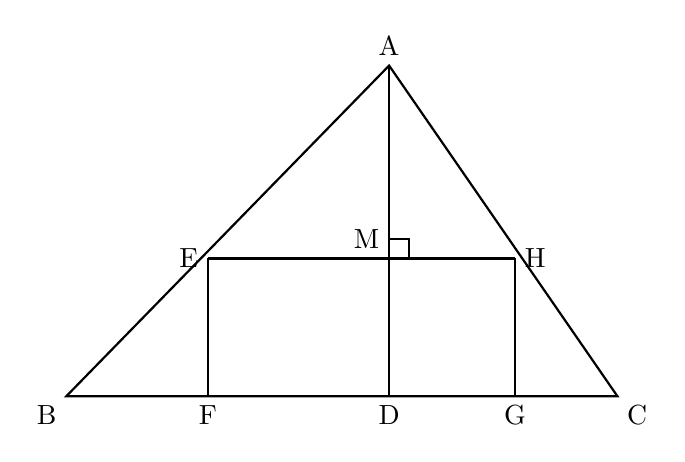
\begin{tikzpicture}[scale=1]
% coordinates
\coordinate (B) at (0,0);
\coordinate (C) at (7,0);
\coordinate (D) at (4.1,0);
\coordinate (A) at (4.1,4.2);
\coordinate (F) at (1.8,0);
\coordinate (G) at (5.7,0);
\coordinate (E) at (1.8,1.75);
\coordinate (H) at (5.7,1.75);
\coordinate (M) at (4.1,1.75);

% triangle sides
\draw[thick] (B) -- (A) -- (C) -- cycle;

% base segments (GD and FB solid, DF dashed)
\draw[thick] (B) -- (F);
\draw[thick,dashed] (F) -- (D);
\draw[thick] (D) -- (C);

% rectangle and altitude
\draw[thick] (E) -- (F);
\draw[thick] (H) -- (G);
\draw[thick] (E) -- (H);
\draw[thick] (A) -- (D);

% right angle mark at M
\draw[thick] ($(M)+(0,0.25)$) -- ($(M)+(0.25,0.25)$) -- ($(M)+(0.25,0)$);

% labels
\node[above] at (A) {A};
\node[below left] at (B) {B};
\node[below] at (F) {F};
\node[below] at (D) {D};
\node[below] at (G) {G};
\node[below right] at (C) {C};
\node[left] at (E) {E};
\node[right] at (H) {H};
\node[above left] at (M) {M};
\end{tikzpicture}
\end{document}
